% -----------------------------------------------------------------------------
% LICENSE: This work is licensed under a Creative Commons Attribution 4.0
% International License (CC BY 4.0). You are free to share and adapt this
% material for any purpose, even commercially, under the condition that you
% give appropriate credit.
% https://creativecommons.org
% -----------------------------------------------------------------------------

\documentclass[10pt, a4paper, oneside]{article}

\usepackage[hidelinks]{hyperref}
\usepackage{jucs2e}
\usepackage{graphicx}
\usepackage{url}
\usepackage{ulem}
\usepackage{mathtools}
\usepackage{scalerel}
\usepackage{setspace}
\usepackage[strict]{changepage}
\usepackage{caption}
\usepackage[letterspace=-50]{microtype}
\usepackage{fontspec}
\usepackage{afterpage}
\usepackage{ragged2e}

\setmainfont{Times New Roman}

\usepackage{titlesec}

\titleformat*{\section}{\Large\bfseries}
\titleformat*{\subsection}{\normalsize\bfseries}

\renewcommand{\baselinestretch}{0.9}

\graphicspath{{./figures/}}

\usepackage[textwidth=8cm, margin=0cm, left=4.6cm, right=4.2cm, top=3.9cm, bottom=6.8cm, a4paper, headheight=0.5cm, headsep=0.5cm]{geometry}
\usepackage{fancyhdr}
\usepackage[format=plain, labelfont=it, textfont=it, justification=centering]{caption}
\usepackage{breakcites}
\usepackage{microtype}

\apptocmd{\frame}{}{\justifying}{}

\urlstyle{same}
\pagestyle{fancy}

\newcommand\jucs{{Journal of Universal Computer Science}}
\newcommand\jucsvol{vol. 27, no. 1 (2021)}
\newcommand\jucspages{2987-2989}
\newcommand\jucssubmitted{1/1/2021}
\newcommand\jucsaccepted{2/2/2021}
\newcommand\jucsappeared{3/3/2021}
\newcommand\jucslicence{ CC BY 4.0}
\newcommand\startingPage{2987}
\setcounter{page}{\startingPage}

%Author
\newcommand\paperauthor{{Voroniy, M.: }}

% Title
\newcommand\papertitle{Using Trie Data Structure for Database Index Representation}

% Main header content
\header{\paperauthor \papertitle}

\begin{document}

\title{{\fontsize{14pt}{14pt}\selectfont{\vspace*{-3mm}\papertitle\vspace*{-1mm}}}}

\author{{\bfseries\fontsize{10pt}{10pt}\selectfont{Maksym Voroniy}} \\
   {\fontsize{9pt}{12pt}\selectfont{(National Technical University «KhPI», Kharkiv, Ukraine\\
   \orcid{0009-0008-7505-5686},
   maksym.voroniy.research@gmail.com)}}
}

\label{first}
\maketitle

{\fontfamily{ptm}\selectfont
\begin{abstract}
{\fontsize{9pt}{9pt}\selectfont{\vspace*{-2mm}
Modern database systems rely heavily on time-proven algorithms for
representing and organizing data on external storage. At the same time,
they must continuously adapt to evolving hardware architectures and
changing business demands - such as horizontal scalability for big data
workloads and the emergence of vector databases driven by the rapid
growth of AI applications.

A vast body of scientific and engineering work has focused on the
adaptation and optimization of well-known tree-based indexing structures
- such as B-trees, B\textsuperscript{+}-trees, B\textsuperscript{*}-trees, and R-trees - to meet these
challenges. These structures have become foundational to modern storage
engines due to their strong performance characteristics on
block-oriented storage systems.

This article, however, aims to draw attention to a different class of
data structures, referred to by Donald Knuth as digital searching
techniques \cite{knuthVol3}. Among these, the Trie (also known as a prefix tree)
occupies a special place. Unlike comparison-based trees, Tries organize
data according to the structure of keys themselves, making them
particularly well-suited for representing and indexing wide range of
digital data not only well known strings, but bit sequences, and encoded
numbers or even vectors.

This article serves as the first in a series exploring how Trie-based
data structures can be applied to address modern, complex indexing
problems. The goal is to demonstrate how Tries enable efficient,
scalable, and structurally expressive representations for arbitrary data
- offering alternative design trade-offs that are increasingly relevant
in contemporary database and data-intensive systems.}}
\end{abstract}}


{\fontfamily{ptm}\selectfont
\begin{keywords}
{\fontsize{9pt}{9pt}\selectfont{
    Trie, Prefix Tree, Database Indexing,
    Memory-Efficient Data Structures, Bitmap Indexing, Page-Oriented Storage
}}
\end{keywords}}

{\fontfamily{ptm}\selectfont
\begin{category}
{\fontsize{9pt}{9pt}\selectfont{
E.1, E.2, E.4, F.2.2, H.2.2, H.3.1}}
\end{category}}

{\fontfamily{ptm}\selectfont
\begin{doi}
{\fontsize{9pt}{9pt}\selectfont{
10.3897/jucs.\textless SubmissionNumber\textgreater}}
\end{doi}}

\section{Introduction}\label{sec1}

Improving the efficiency of a data structure does not necessarily require replacing its fundamental algorithm. In many practical cases, the largest gains can be achieved by reconsidering how the existing structure is represented in memory.

Trie-based structures provide a particularly illustrative example. A straightforward Trie implementation can represent each node as a fixed-size lookup table indexed by the alphabet. Such a representation provides constant-time navigation, but its memory consumption is proportional to the size of the alphabet rather than to the actual number of children of a node. For sparsely populated nodes, the majority of the allocated space therefore represents absent edges.

A common approach to this problem is to introduce progressively more sophisticated node representations: hash tables, sorted arrays, or adaptive node types selected according to the number of stored children. These techniques improve the utilization of allocated memory, but they still leave an important question: what is the appropriate unit at which the optimization should be applied?

This work follows a different principle. Rather than making small, isolated modifications to the Trie algorithm, it treats the node representation itself as an optimization target. In particular, the proposed approach separates the identification of existing edges from their physical storage. A compact bit-indexed structure can represent the presence of children over the complete alphabet, while a contiguous array stores only the actually existing entries. This makes it possible to preserve constant-time navigation and ordered traversal while avoiding the space cost of empty lookup-table entries.

The objective is therefore not to propose a radically different indexing algorithm, but to demonstrate how small changes in the representation at the right structural level can produce substantial improvements in memory efficiency of the Trie. The following sections develop this idea from the basic Trie representation through sparse-node compression, bit-indexed navigation, and specialized root handling.


\section{Results}\label{sec2}

\begin{itemize}
\item Introduced a step-by-step approach to formalizing the Trie data structure as a foundation for further research.
\item Proposed a space-efficient node representation based on bitmap indexing and compact arrays for sparsely populated Trie nodes.
\end{itemize}

\section{Informal Trie introduction}\label{informal_intro}

A Trie, also known as a prefix tree or digital tree, is a tree-based data structure
originally developed for storing and efficiently retrieving strings. Unlike
comparison-based search trees, where a complete key is typically stored in a node
and compared with other keys, a Trie represents a key by a path from the root through a sequence of nodes.

The simplest - though informal - way to introduce the Trie data
structure is to start by grouping several strings and observing their
shared prefixes. Consider the following set of words:

\{car, cart, computer, cat\}

The common prefix for all words is "c". The words "car", "cart", and
"cat" additionally share the prefix "ca", while "car" itself is a common
prefix of "car" and "cart".

Figure~\ref{fig:3word} illustrates the corresponding prefix tree constructed from this
set of words.


\begin{figure}[h]
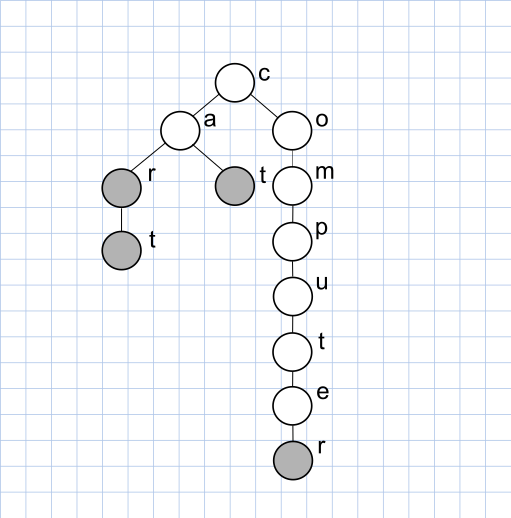
\includegraphics[width=0.85\textwidth]{01.3-word}
\centering
\captionsetup{font=small}
\caption{\fontsize{10pt}{11pt}\selectfont{\itshape{Simple prefix tree}}}
\label{fig:3word}
\end{figure}

This example highlights several important concepts fundamental to
Trie-based structures that are reviewed in details in the following sections.

\subsection{Terminal and Non-terminal
Nodes}\label{terminal-and-non-terminal-nodes}

A prefix tree constructed by combining all possible characters
implicitly represents a large number of non-existing words, such as
"co", "ca", or "comp". To distinguish valid keys from such intermediate
prefixes, the diagram marks only existing words using a visual indicator
(shown in grey).

A node corresponding to the final character of an existing word is
marked as terminal, while nodes representing prefixes that are not
complete words are considered non-terminal. As illustrated by the words
"car" and "cart", a terminal node does not necessarily have to be a leaf
node. Conversely, every leaf node is necessarily terminal.

\subsection{Structural Redundancy and Space
Usage}\label{structural-redundancy-and-space-usage}

Another aspect that becomes immediately apparent in Figure~\ref{fig:3word} is the
potential inefficiency in space usage. For example, the word "computer"
introduces a long substring "ompute" that is unique and therefore stored
as a linear chain of nodes. This can result in a significant number of
nodes that do not contribute to shared structure.

This issue will be addressed later when the Trie is defined more
formally. In particular, the PATRICIA (Practical Algorithm to Retrieve
Information Coded in Alphanumeric) approach \cite{HIMANSHU_CHATURVEDI_BANDYOPADHYAY_JAIN_2017} demonstrates how
such linear chains can be compressed, significantly reducing the number
of nodes required.

At this stage, it is important to distinguish between a node and an
encoded character. A node is an element of the data structure that:

\begin{itemize}
\item
  may represent one or more characters,
\item
  contains a terminal/non-terminal indicator,
\item
  and may hold references to child nodes.
\end{itemize}

\subsection{Root Expansion and Node
Structure}\label{root-expansion-and-node-structure}

A third important observation arises when adding a string that does not
share the existing root prefix. For example, consider inserting the
word:

\bigskip
      \{art\}
\bigskip

Since the letter "a" is not part of any existing prefix, the root node
must be extended to include an additional branch.

\begin{figure}[h]
    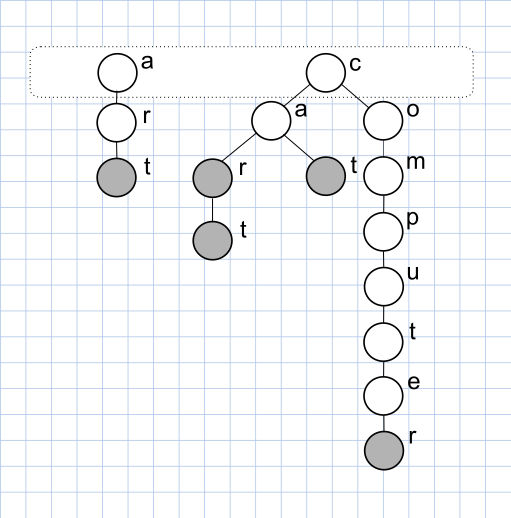
\includegraphics[width=0.85\textwidth]{02.5-word}
    \centering
    \captionsetup{font=small}
    \caption{\fontsize{10pt}{11pt}\selectfont{\itshape{Crafting root node}}}
    \label{fig:5word}
\end{figure}

This operation raises an essential design question: what is the internal
structure of a Trie node? The need to accommodate multiple starting
characters at the root level makes explicit the role of nodes as
branching points rather than mere containers for characters.

\section{Formal definition}\label{formal-definition}

The formal definition of a Trie is based on several fundamental concepts.
First, an alphabet defines the set of symbols that can be used to construct keys.
A key defines an ordered sequence of such symbols, while a node defines the structural elements
used to represent these sequences as paths in the Trie. These concepts are introduced step by step
in the following sections.

\subsection{Alphabet}\label{alphabet}

In the context of this article, an alphabet \(\Sigma\) is a finite, non-empty set of distinct symbols
that can be used to construct Trie keys. A symbol is the smallest indivisible element considered by
the Trie when navigating from one node to another.

Formally,
\begin{equation}
\Sigma = {b_1, b_2, \ldots, b_n}, \qquad |\Sigma| = n > 0.
\end{equation}

The alphabet does not necessarily represent a natural-language alphabet. It defines the set of
possible values that may occur at each position of a key. Consequently, the choice of alphabet depends
on how the indexed data is represented.
The unary case, \(n=1\), is mathematically valid but represents a degenerate Trie in which every node
has at most one outgoing edge. Consequently, the Trie forms a single chain and provides no branching-based
search advantage. The practically relevant cases considered in this article therefore have \(n > 1\).

Table~\ref{tab:alphabetExamples} presents several alphabets relevant to the representations considered in this
and subsequent articles.


\begin{table}[ht]
    \centering
    \setlength\tabcolsep{6pt}
\begin{tabular}{|l|l|l@{}|}
\hline
\bfseries Example & \bfseries Set definition &
    \begin{tabular}{l}
    \bfseries Set cardinality \\
    \bfseries (alphabet power)
    \end{tabular} \\
\hline
% 1.
Boolean values - binary alphabet &
$\Sigma_{2} = \left\{ 0,1\right\}$ &
$\left| \Sigma_{2} \right| = 2$ \\
% 2.
Small English letters &
\(\Sigma_{26} = \{ a,b,\dots z\}\) &
\(\left| \Sigma_{26} \right| = 26\) \\
% 3.
Unsigned 8-bit integer  &
\(\Sigma_{byte} = \{ 0,1,\dots255\}\) &
\(\left| \Sigma_{byte} \right| = 256\) \\
% 4.
Signed 8-bit integer &
\(\Sigma_{i128} = \{ - 128,\dots127\}\)&
\(\left| \Sigma_{i128} \right| = 128\) \\
\hline
\end{tabular}
    \caption{\fontsize{10pt}{11pt}\selectfont{
        \itshape{Examples of alphabets}
    }}
    \label{tab:alphabetExamples}
\end{table}
\noindent

For example, \(\Sigma_{26}\) can represent the 26 lowercase English letters, that was used in previous chapter
during non-formal definition of Trie. While \(\Sigma_{byte}\) can represent
all 256 possible byte values. The latter is particularly relevant for computer-oriented string representations,
including UTF-8, where a string can be processed as a sequence of bytes.

The alphabet used by a Trie therefore defines its branching domain: for every key position, the next symbol must belong
to \(\Sigma\). The size of this alphabet has a direct impact on the memory requirements of node representations, which
becomes particularly important when a node is implemented as a fixed-size lookup table.

\subsection{Key}\label{key}

A key is a finite non-empty sequence of symbols from $\Sigma$:

\begin{equation}
k = b_{1},b_{2} \ldots,
 \mathrm{where}\!:
  b_{i} \in \Sigma  \land  i > 0
\end{equation}

Since this article focuses on the practical use of Tries for database
indexing, a key is not sufficient on its own. Each key must be
associated with a value. Let $V$ denote an arbitrary value domain - such
as integers, floating-point numbers, strings, or, in subsequent
articles, vectors.

A Trie therefore represents a key - value mapping, where a value
\(v = V\) is associated with a key $k$ at its terminal position in the
structure.

\subsection{Node}\label{node}

Throughout this article, a Trie has been described as a tree, which in
turn is a special case of a graph. A graph consists of nodes and edges,
and the following discussion clarifies how these concepts are
interpreted in a Trie designed for practical use in key-value
databases.

The vast majority of modern database indexing structures are based on
B-tree variants, most notably B-trees, B\textsuperscript{+}-trees, and B\textsuperscript{*}-trees \cite{zhang2022memory,idreos2019design}.
      On the one hand, this dominance can be explained by the existence
of mature, well-understood algorithms supporting insertion, deletion,
point queries, and range queries. On the other hand, it is equally
important to consider the influence of modern hardware architectures.

B-tree - based indexes are closely aligned with page-oriented access
patterns, which efficiently exploit hardware mechanisms such as Direct
Memory Access (DMA) and Ultra DMA (UDMA) for transferring large
contiguous blocks of data between storage devices, memory, and
processors \cite{fent2020low,vogel2023towards,lasch2024heterogeneous}.
By organizing nodes as disk-sized pages, these
structures minimize I/O operations and achieve high throughput on
external storage.

In contrast, most academic definitions of Tries do not explicitly
address page-organized access. Instead, they typically assume
fine-grained, pointer-based node representations. To bridge this gap, we
begin with a conventional node definition and later extend it to better
exploit page-oriented storage.

\subsection{Root Node and Navigation}\label{root-node-and-navigation}

As defined in classical sources \cite{knuthVol3, fds_alg}, a Trie contains a
distinguished root node corresponding to the empty key $\epsilon$. All operations
on the Trie begin at this root.
However, the empty string is not considered a valid key in the
data model used in this work. Consequently, the root does not need to represent
a separate key value. This observation allows the conventional non-functional
root to be replaced by a root node that participates in the same representation as the other
nodes. In particular, the root can contain the payload associated with the first level
of the Trie rather than serving solely as a structural entry point.
The motivation is not merely to eliminate one node. More importantly, treating
the root as an ordinary functional node reduces the number of special cases in subsequent
algorithms. When all nodes follow the same representation and expose the same operations,
algorithms can be expressed at a finer and more uniform granularity: traversal, lookup,
insertion, and node optimization can be defined in terms of a single node abstraction rather than requiring
separate processing for the root. Thus, the distinction between the root and other nodes is not required
by the semantics of the key set, but is primarily a consequence of the conventional representation.
Since the empty string is outside the considered key domain, this distinction can be removed without
changing the set of represented keys.

With the Trie representation established, we can define the lookup operation in terms of a mapping
from a key to either its existence status or its associated value. The simplest form of this
operation is the \textit{Exists} predicate, which determines whether a given key is represented by a terminal
node in the Trie:

\begin{equation}
E(k) \rightarrow \{\mathrm{True},\mathrm{False}\}.
\end{equation}

For the Trie depicted in Figure~\ref{fig:5word}, the predicate evaluates as follows:

\begin{table}[ht]
    \centering
    \setlength\tabcolsep{6pt}
    \begin{tabular}{|l|p{0.7\linewidth}| }
    \hline
    \bfseries Query & \bfseries Result \\
    \hline
    % 1.
    \(E("art")\) & True \\
    % 2.
    \(E("car")\) & True \\
    % 3.
    \(E("ca")\) & False (no such terminal) \\
    % 4.
    \(E("camp")\) & False \\
    \hline
    \end{tabular}
    \caption{\fontsize{10pt}{11pt}\selectfont{
        \itshape{Sample evaluation of Exists (\(E\)) predicate.}}
    }
    \label{tab:queryExists}

\end{table}
\noindent


The definition above describes the \textit{result} of a lookup, but does not specify how
this result is obtained. The next question is therefore the computational cost of evaluating $E(k)$.
In particular, the lookup procedure must determine, for each successive symbol of the key, whether
the corresponding outgoing edge exists. The complexity of this operation depends directly on how
the outgoing edges of each Trie node are represented.


\subsubsection{Lookup Complexity with Linear Edge Scanning}
\label{lookup-complexity-with-linear-edge-scanning}

Let us analyze the complexity of the lookup operation \cite{largescalesearch2021} using a naive node representation.
Consider the worst-case scenario in which the requested key does not exist in the Trie, for example, "can".

\begin{enumerate}
  \def\labelenumi{\arabic{enumi}.}
\item Start at the root node.
\item Iterate over all outgoing edges of the root and compare their labels with the first symbol, "c".
 The edge labeled "c" is found.
\item Move to the child corresponding to "c".
Iterate over its outgoing edges and compare their labels with the second symbol, "a". The edge labeled "a" is found.
\item Move to the child corresponding to "a".
Iterate over its outgoing edges and compare their labels with the third symbol, "n" that does not match to any, and
the search terminates with \texttt{False}.
\end{enumerate}


If a node has $N$ outgoing edges, finding a matching edge by linear scanning requires $O(N)$ time.
For a key containing $m$ symbols, the lookup may have to perform such a search at each level of the Trie.
Let $N_i$ denote the number of outgoing edges at the node visited at level $i$. The total lookup complexity is therefore

\begin{equation}
O(N_1 + N_2 + \dots + N_m).
\end{equation}

In the worst case, when each visited node has approximately $N$ outgoing edges, this becomes $O(mN)$.

An obvious improvement is to keep the outgoing edges sorted by their labels. This allows binary search at each node
and reduces the lookup complexity to

\begin{equation}
O(\log N_1 + \dots + \log N_m),
\end{equation}

However, an even more direct approach is to eliminate the need for edge scanning altogether by mapping each
symbol to a predetermined position. This leads to the lookup-table representation described in the following section.

\subsubsection{Lookup Table}
\label{lookup-table}

A common optimization is to provide each node with a lookup table indexed by the alphabet $\Sigma$. In this
representation, as depicted in Figure~\ref{fig:lookupTable}, each possible symbol corresponds to a fixed
slot containing either a reference to a child node or an empty value (\texttt{nil}). So applying lookup table allows:

\begin{itemize}
\item
  to achieve constant-time of child selection,
\item
  to travers directly node symbols \(b_{1},b_{2}\ \dots b_{m}\),
\item
  eliminated search iteration over outgoing edges.
\end{itemize}


\begin{figure}[h]
    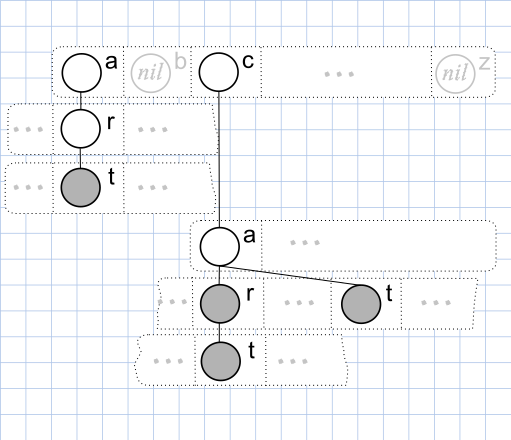
\includegraphics[width=0.85\textwidth]{03.lookup-table}
    \centering
    \captionsetup{font=small}
    \caption{\fontsize{10pt}{11pt}\selectfont{\itshape{Lookup table example for \(\Sigma_{26}\) alphabet}}}
    \label{fig:lookupTable}
\end{figure}

As a result, the complexity of the Exists predicate becomes:

\begin{equation}
O(1 + 1 + \dots + 1) = O(m).
\end{equation}


An additional benefit of this approach is its compatibility with
page-organized access. Fixed-size tables align naturally with cache
lines and memory pages, making this representation more amenable to
high-throughput, hardware-efficient implementations than pointer-heavy,
irregular node layouts.

Another important property of lookup-table based Trie nodes is that
traversal algorithms can rely on a fixed, globally ordered alphabet
within a single page. This guarantees deterministic navigation across
levels of the Trie and enables efficient, branch-free lookup logic.
Later in this article, we will show how this property can be exploited
to improve navigation and traversal performance.

The major drawback of lookup tables, however, is their memory
inefficiency when nodes are sparsely populated. In many cases, a large
fraction of table entries remain unused, yet still consume memory. This
issue becomes particularly visible when indexing natural-language data.

Consider English words over an alphabet \(\Sigma_{26}\). As demonstrated
in prior studies \cite{yau2014distribution, norvig2012english} , English spelling rules forbid most letter
combinations. For example, a word starting with the letter "q" is almost
always followed by "u", creating a strong statistical bias at the second
level of the Trie. As a result, a lookup table allocated for all 26
possible successors at that level will be overwhelmingly empty, leading
to poor space utilization.

Consequently, lookup-table based nodes can be highly inefficient for
sparse or skewed alphabets. This observation motivates the exploration
of alternative representations - most notably hash tables and sorted
arrays - which trade constant-time access for improved space efficiency.
The next section examines these alternatives and analyzes their impact
on lookup performance and memory layout.

\subsubsection{Page Space Optimization}\label{page-space-optimization}

To overcome the space inefficiency of lookup-table - based nodes, we
need to select alternative data structures that satisfy the following
requirements:

\begin{itemize}
\item
  Access complexity better than \(O(N)\) for locating an element
  \(b_{i}\).
\item
  Compatibility with page-based access, favoring linear or contiguous
  memory layouts. (For this reason, linked lists are poor candidates.)
\item
  Support for ordered navigation, which is desirable for prefix scans
  and range-like traversal.
\item
  Space usage significantly smaller than the alphabet size, i.e.:
\begin{equation}
l \ll |\Sigma|.\label{eq:lessThanAlphabet}
\end{equation}

Otherwise, a full lookup table indexed by \(\Sigma\) remains the optimal solution.

\end{itemize}


A widely adopted memory-saving technique is to combine full lookup
tables for densely populated nodes with compact control structures for
sparse nodes. This idea is formalized in the family of data structures
commonly referred to as adaptive Tries or Adaptive Radix Trees
(ART) \cite{leis2013adaptive}.

The core principle is simple: node representations adapt to their
fan-out (population size). When the number of outgoing edges is small,
compact representations are used; as the node becomes denser, the
representation gradually expands. In practice, this expansion is often
performed in powers of two, for example, arrays of size 8, 16, 32, and
so on, until condition (\ref{eq:lessThanAlphabet}) is violated and a full lookup table becomes
justified.

Some approaches \cite{farachcolton2025optimalboundsopenaddressing} propose the use of hash tables with open
addressing for sparse nodes. While effective for lookup, hash tables
lack inherent ordering and introduce additional complexity. Instead, we
can craft a custom node representation that satisfies all previously
stated requirements: fast lookup, ordered navigation, linear memory
layout, and efficient space usage.

We begin with a bitmap that encodes the presence or absence of outgoing
edges. Each bit corresponds to one symbol \(b_{i}\) .

\begin{itemize}
\item
  bit value 1 - means corresponding child exists
\item
  bit value 0 - means no child for that symbol.
\end{itemize}

The bitmap size exactly matches the alphabet size \(|\Sigma|\).
The Exists predicate \(E\left( b_{i} \right)\) is implemented
by a single bit test, yielding constant-time performance. For example,
at Figure~\ref{fig:adaptiveSizedNodes}, symbols "a" and "c" correspond to bits set to 1, while "b"
and "z" correspond to bits set to 0.

\begin{figure}[h]
    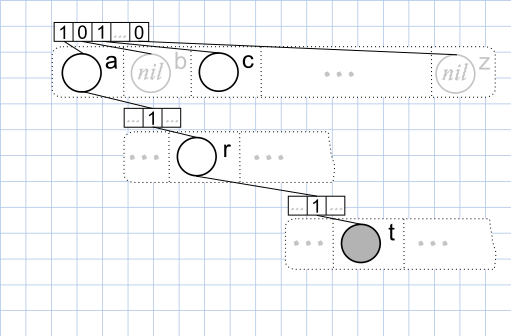
\includegraphics[width=0.85\textwidth]{04.Adaptive-sized-nodes}
    \centering
    \captionsetup{font=small}
    \caption{\fontsize{10pt}{11pt}\selectfont{\itshape{Combine bitmap with array}}}
    \label{fig:adaptiveSizedNodes}
\end{figure}

Modern processors efficiently support bitmap operations using native
integer registers. For an alphabet
\(\left| \Sigma_{byte} \right| = 256\), the bitmap requires only four
64-bit unsigned integers, representing a negligible memory overhead.

To store associated child references or service metadata, the bitmap is
paired with a compact ordered array (Figure ~\ref{fig:bitmapAndArray}). This array stores only
the existing children, eliminating all (\texttt{nil}) entries present in full
lookup tables.

  Key properties of this design:
\begin{itemize}
\item
  The bitmap provides $O(1)$ existence checks.
\item
  The array stores only populated entries.
\item
  Array elements are maintained in sorted order, enabling ordered
  traversal.
\item
  The index into the array is computed using a population count
  (popcount\footnote{
The vast majority of modern CPUs support the POPCNT instruction
 for calculating the rank of a set bit
}) over the bitmap.
\end{itemize}

As a result, this structure removes wasted space while preserving fast
access and ordered navigation.

\begin{figure}[h]
    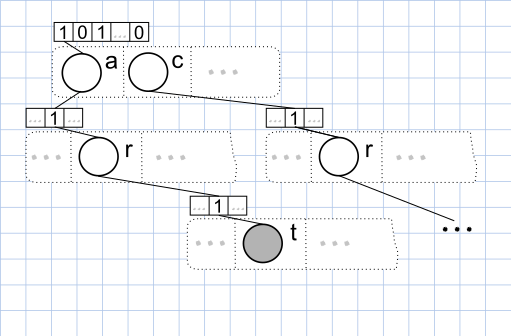
\includegraphics[width=0.85\textwidth]{05.Bitmap-and-Array}
    \centering
    \captionsetup{font=small}
    \caption{\fontsize{10pt}{11pt}\selectfont{\itshape{Using array of bitmap for lookup}}}
    \label{fig:bitmapAndArray}
\end{figure}


Summarizing the properties of this bitmap-array let's articulate:
\begin{itemize}
    \item
      Bitmap operations are directly supported by native CPU instructions.
    \item
      Compact arrays minimize memory footprint while maintaining linear space complexity.
    \item
      Alphabet ordered traversal remains natural and efficient.
    \item Lookup has $O(1)$ complexity for a fixed-size alphabet.
\end{itemize}

\subsection{Wrapping things up}\label{wrapping-things-up}

The preceding analysis shows that lookup efficiency ultimately
depends on how a symbol $b_i$ is mapped to an outgoing edge of a Trie node.
At its core, the Trie algorithm implements a mapping
between key elements and edges of a graph, which is the fundamental
structural principle of the Trie data structure. Let $T$ be set of all Trie nodes. Then Trie
defines a transition function that, for a given node \(n \in T\) and a symbol \(b \in \Sigma\),
selects the outgoing edge labeled by $b$ and returns the corresponding
child node or (\texttt{nil}).

\begin{equation}
f:T \times \Sigma \rightarrow T \cup \{\bot\}
\end{equation}

Intuitively, \(f(n,~b)\) answers the question: ``From node
$n$, where do we go when we read symbol $b$?''

\begin{equation}
f(n,~b)= \Biggl\{
\begin{array}{ll}
    n, & \text{if an edge } n \xrightarrow{\text{b}}n' ~exists,\\
    \bot, & \text{otherwise}.
\end{array}\label{eq:mappingFunction}
\end{equation}


Since a key is a sequence of symbols \(b_1, b_2\dots b_m\), repeated application of this
transition function defines a mapping from keys to nodes of the graph. Starting from the
root node, we can define the traversal function F as a composition of transitions:

\begin{equation}
    \begin{array}{ll}
     F: \oslash  \rightarrow \bot \\
     F: \left\{ b_{1},b_{2}\ \dots b_{m} \right\} \rightarrow f( b_{1} ) \circ f(b_{2}) \circ \dots f(b_{m})
\end{array}\label{eq:composeLetterMap}
\end{equation}

With this in mind, a Trie can be formally defined as a tuple:

\begin{equation}
Trie \coloneqq < \Sigma, T, E, \mathrm{root}, f >
\end{equation}

where:

\begin{itemize}
\item
  $\Sigma$ is a finite alphabet,
\item
  $T$ is a set of nodes,
\item
  \(E \subseteq T \times \Sigma \times T\) is a set of labeled edges,
\item
  \(root \in T\) is the root node, where lookup is starting,
\item
  \(f:T \times \Sigma \rightarrow T \cup \{\bot\}\), is a transition
  function consistent with $E$.
\end{itemize}

Under this definition, the Trie is a rooted, tree-like graph in which
the function $F$ (\ref{eq:composeLetterMap}) maps any key, represented as a sequence of symbols
from $\Sigma$ to a unique node in $T$ by following the corresponding labeled
path from the root.

This formal representation also provides a basis for practical key-value retrieval.
Nodes and edges can be equipped with additional information, allowing the mapping $F$ to be extended
from locating a key to retrieving its associated value and other structural metadata.

      \subsubsection{Value retrieving}\label{value-retrieving}

      Following the logic represented in (\ref{eq:mappingFunction}) association of value $v$ with key $k$ can be
      expressed as:
\begin{equation}
Val(k)= \Biggl\{
\begin{array}{ll}
    v, & \text{if}~k~\text{present},\\
    \bot, & \text{otherwise}.
\end{array}\label{eq:mappingValue}
\end{equation}

      \subsubsection{Structural metadata retrieving}\label{meta-retrieving}
The properties of the data structures discussed in this article allow certain types of
metadata to be obtained directly from the representation. In particular, for a node corresponding
to a prefix $P$, the bitmap and ordered child array provide the following operations:

\begin{itemize}
\item \textbf{Count child items.}
The number of immediate child edges of a prefix can be obtained directly from the bitmap using a population-count
operation such as \texttt{POPCNT}. Thus, the branching factor of a prefix can be determined without traversing
its child array.
\item \textbf{Check key existence.}
The bitmap provides a direct basis for implementing the \textit{Exists} predicate introduced earlier.
Testing the corresponding bit determines whether an edge labeled by a given symbol exists, while the rank of the
set bit identifies its position in the compact child array.

\item \textbf{Retrieve minimum and maximum child symbols.}
Because the bitmap represents symbols according to the intrinsic order of the alphabet, the minimum and maximum
existing child symbols can be determined directly by locating the first and last set bits. No additional ordering
structure or traversal of the child array is required.

\item \textbf{Retrieve minimum and maximum keys.}
Starting from any node, including the root or a node representing a prefix $P$, repeatedly selecting the child with
the minimum symbol leads to the lexicographically smallest terminal key in that subtree.
Similarly, repeatedly selecting the child with the maximum symbol leads to the lexicographically largest terminal key.
Thus, minimum and maximum keys for an arbitrary prefix can be obtained through a deterministic traversal without
requiring a separate ordering structure.

\end{itemize}


\section{Conclusion}
\label{conclusion}

This article examined the Trie as a data structure for database indexing, starting from its classical use for
storing and retrieving strings and progressively developing a formal representation suitable for practical
implementation. The analysis focused on the fundamental operation of mapping a key symbol to the corresponding
outgoing edge of a Trie node and showed how the representation of this mapping directly affects lookup
complexity and memory consumption.

Several alternative representations were considered, including linear edge scanning, ordered arrays,
direct lookup tables, and compact bitmap-arrays. The proposed bitmap-array representation separates the
identification of existing edges from their physical storage: a bitmap represents the presence of symbols in the
alphabet, while a compact ordered array stores only the corresponding child nodes. This allows sparse nodes to
avoid allocating storage for absent edges while retaining constant-time lookup for a fixed-size alphabet
and natural alphabet-ordered traversal.

The analysis also showed that the proposed representation provides properties beyond memory optimization.
The bitmap can serve as a source of structural information, allowing the number of immediate children to be
obtained through population counting, supporting the \textit{Exists} predicate and \textit{Val} function, and providing
direct access to minimum and maximum child symbols. Combined with ordered traversal, these properties also allow the
lexicographically minimum or maximum key of an arbitrary prefix subtree to be located without requiring
a separate ordering structure.

\begin{thebibliography}{}{
\fontsize{9pt}{10pt}\selectfont

\bibitem[Knuth. 1998]{knuthVol3}Knuth, D.E.: The Art of Computer Programming, Volume 3: Sorting and
Searching, 2nd edn. Addison-Wesley, Reading, Mass. (1998)

%%% 2
\bibitem[HIMANSHU et~al. 2017]{HIMANSHU_CHATURVEDI_BANDYOPADHYAY_JAIN_2017}HIMANSHU, CHATURVEDI, K.K., BANDYOPADHYAY, A., JAIN, S.: Patricia trie based time and memory optimization for fast network motif search. The
Indian Journal of Animal Sciences 87(4), 512–519 (2017) \url{https://doi.org/10.
56093/ijans.v87i4.69625}

%%% 3
\bibitem[Zhang et~al. 2022]{zhang2022memory} Zhang, H., Chen, S., Carey, M.: Memory-efficient and cache-friendly indexing for
modern database systems. The VLDB Journal 31(6), 1245–1267 (2022)


%%% 4
\bibitem[Idreos et~al. 2019]{idreos2019design}Idreos, S., Dayan, N., Qin, W., Akmanalp, M., Hilgard, S., Ross, A.,
Lennon, J., Jain, V., Gupta, H., Li, D., Zhu, Z.: Design continuums
and the path toward self-designing key-value stores that know and learn.
(2019). \url{https://stratos.seas.harvard.edu/publications/design-continuums-and-pathtoward-self-designing-key-value-stores-know-and}


%%% 5
\bibitem[Fent et~al. 2020]{fent2020low}Fent, P., Renen, A., Kipf, A., Leis, V., Neumann, T., Kemper, A.: Low-latency
communication for fast dbms using rdma and shared memory. In: 2020 IEEE 36th
International Conference on Data Engineering (ICDE), pp. 1477–1488 (2020).
\url{https://doi.org/10.1109/ICDE48307.2020.00131}.


%%% 6
\bibitem[Vogel et~al. 2023]{vogel2023towards} Vogel, L., Hilprecht, B., Binnig, C.: Towards foundation models for relational
databases [vision paper]. arXiv preprint arXiv:2305.15321 (2023)

%%% 7
\bibitem[Lasch. 2024]{lasch2024heterogeneous}Lasch, R.: Heterogeneous memory technologies in database management systems.
PhD thesis, Technische Universit¨at Ilmenau, Ilmenau, Germany (2024). \url{https:
//doi.org/10.22032/dbt.62299}

%%% 8
\bibitem[Nipkow. 2025]{fds_alg}Nipkow, T. (ed.): Functional Data Structures and Algorithms: A Proof Assistant
Approach vol. 67, 1st edn. Association for Computing Machinery, New York, NY,
USA (2025)

%%% 9
\bibitem[Feng et~al. 2021]{largescalesearch2021}Feng, D., Liang, M.-G., Gao, F., Huang, Y.-C., Zhang, X.-F., Duan, L.-Y.:
Towards large-scale object instance search: A multi-block n-ary trie. IEEE Transactions on Circuits and Systems for Video Technology 31(1), 372–386 (2021)
\url{https://doi.org/10.1109/TCSVT.2020.2966541}

%%% 10
\bibitem[Yau. 2014]{yau2014distribution}Yau, N.: Distribution of letters in the English language. Accessed:
September 7, 2026 (2014). https://flowingdata.com/2014/06/01/
distribution-of-letters-in-the-english-language

%%% 11
\bibitem[Norvig. 2012]{norvig2012english}Norvig, P.: English Letter Frequency Counts: Mayzner Revisited or ETAOIN
SRHLDCU. \url{https://norvig.com/mayzner.html}. Accessed: September 7, 2026
(2012)

%%% 12
\bibitem[Leis et~al. 2013]{leis2013adaptive} Leis, V., Kemper, A., Neumann, T.: The adaptive radix tree: Artful indexing
for main-memory databases. In: 2013 IEEE 29th International Conference on
Data Engineering (ICDE), pp. 38–49 (2013). \url{https://doi.org/10.1109/ICDE.2013.
6544812}. IEEE

%%% 13
\bibitem[Farach-Colton  et~al.2025]{farachcolton2025optimalboundsopenaddressing}Farach-Colton, M., Krapivin, A., Kuszmaul, W.: Optimal Bounds for Open
Addressing Without Reordering (2025). \url{https://arxiv.org/abs/2501.02305}

}\end{thebibliography}



\end{document}
